\begin{beispiel}[Logistisches Wachstum (gebremst)]
\mbox{}\\
$u(t) $ sei Größe einer Population. Nun berücksichtigen wir  hemmende Faktoren wie beschränkte Resourcen, Krankheiten, Kriege oder ähnliches. Wir treffen folgende \textbf{Modellannahme:} Wegen beschränkter Kapazität kann $u(t) $
eine gewisse Maximalgröße $M$ nicht überschrieten und
$\Delta u $ ist proportional zu $u, \ M-u, \ \Delta t$, das heißt
\begin{equation*}
\Delta u = \alpha u(M-u) \Delta t 
\end{equation*}
Wir bereits zuvor machen wir wieder den Grenzübergang
\begin{equation*} 
u' = \gamma u - \tau u^2 \ \ \mathrm{mit\ }\gamma = \alpha M, \ \tau = \alpha
\end{equation*}  
Interpretation: Wachstum $u$ wird durch Term $-\tau u^2 $ für große $u$ 
stärker gebremst als für kleine $u$. \\

Die allgemeine Lösung für $u(0) = u_0 $ ist
\begin{equation*}
u(t) = \frac{\gamma}{\tau + \left(\frac{\gamma}{u_0} - \tau \right) e^{-\gamma t}}
= \frac{M}{1+\left(\frac{M}{u_0} - 1 \right) e^{-\gamma M t}}
\end{equation*}

Seien nun $\alpha, M > 0$ Dann konvergiert $u(t) \xrightarrow{t\rightarrow\infty} M $. Wenn $u_0 \in (0,M)$ ist, dann erhalten wir
\begin{center}
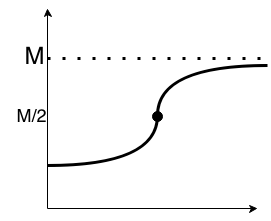
\includegraphics[scale=0.5]{pictures/011-01.png}
\end{center}
und wenn $u_0 >M$, so handelt erhalten wir folgendes
\begin{center}
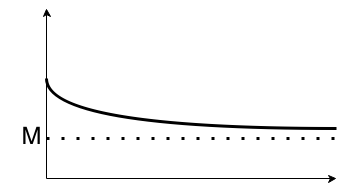
\includegraphics[scale=0.5]{pictures/011-02.png}
\end{center}

Setzen wir $u_0 = M$, so wird $u(t) = M \forall t $ \\

Insbesondere beschreibt logistisches Wachstum:
\begin{itemize}
    \item Gewichtszunahme
    \item Höhenwachstum von Sonnenblumen
    \item Verbreitung von Gerüchten
\end{itemize}

\end{beispiel}
\newpage
\begin{beispiel}[Freier Fall]

Nun sei $v(t) = u'(t) $ die Geschwindigkeit einer Masse $m$. Die 
\textbf{Modellannahme} ist das \emph{Newtonsche Kraftgesetz}: 
\begin{equation*}
K = m u'' 
\end{equation*}
\begin{center}
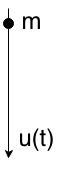
\includegraphics[scale=0.5]{pictures/011-03.png}                        
\end{center}
Die Schwerkraft nahe der Erdoberfläche lässt sich durch $K = mg$ ($g$ - 'Gravitationskonstante') approximieren. Die 
Differenzialgleichung lautet dann
\begin{equation*}
u'' = g \ \ \mathrm{bzw.\ \ }v' = g
\end{equation*}
mit der Lösung
\begin{equation*}
v(t) = v_0 + gt
\end{equation*}
\begin{equation*}
u(t) = u_0 + v_0 t + \frac{1}{2} g t^2
\end{equation*}

Offenbar liefert Vorgabe von $u(0) = u_0 $ und $u'(0) = v_0 $ eine eindeutige Lösung
der Differenzialgleichung (Anfangswertproblem).\\
Alternativ könnte man $u(0) = u_0 $ und $u(t_1) = u_1 $ vorschreiben und erhalten so
\begin{equation*}
\Rightarrow u_1 = u_0 + v_0 t_1 + \frac{1}{2} g t_1^2
\end{equation*}
\begin{equation*}
v_0 = \frac{u_1 - u_0 - \frac{1}{2} g t_1^2}{t_1}
\end{equation*}
Das heißt, man erhält wieder eine eindeutige Lösung (Randwertproblem).
\end{beispiel}
\newpage
\textbf{Wichtige Fragestellungen bei Behandlung von Differenzialgleichungen}\\
\begin{itemize}
    \item \emph{Existenz einer Lösung}
        \begin{itemize}
            \item explizite Lösungen findet man nur in einigen Spezialfällen\\
                ($\rightarrow $ Näherungslösung mittels Computer)
            \item 
                \emph{aber} Existenz einer Lösung kann 
                sehr allgemein abstrakt gezeigt werden (zumindest lokal)
        \end{itemize}
        $\Rightarrow $\emph{qualitative Untersuchungen} 
        der nicht explizit bekannten Lösungen spielen eine wichtige Rolle,
        zum Beispiel:
        \begin{itemize}
            \item Fortsetzunge
            \item Asymptotisches Verhalten
            \item Stabilität
            \item Regularität
            \item Periodizität
            \item ...
        \end{itemize}
    \item \emph{Eindeutigkeit einer Lösung}
        \begin{itemize}
            \item obige Beispiele zeigen, dass idR Parameter auftreten,
                 woraus unendlich viele Lösungen folgen
            \item durch Vorgabe von geeigneten Anfangswerten $(u(0), \ u'(0), \ldots)$
                bzw. von geeigneten  Randwerten $(u(t_0) = u_0, (u(t_1) = u_1) $ 
                ergibt sich häufig eine  eindeutige Lösung
            \item manche Probleme haben in natürlicher Weise keine eindeutige Lösung,
                z.B. Beulprobleme
        \end{itemize}
    \item \emph{Stetige Abhängigkeit der Lösung von Parametern} \\
        Parameter = Anfangswerte, Koeffizienten\\
        Problem: Parameter sind nie exakt messbar! Geringfügige Abweichungen können
        in (chaotischen) Systeme zu völlig unterschiedlichen Lösungen führen 
        (z.B. Doppelpendel). \\
        'Das ist eine ganz wichtige Sache, muss man wissen!'\\
        $\Rightarrow $ kleine Störung der Parameter sollten nur 
        kleine Veränderung der Lösung bewirken, d.h. die Lösung sollte stetig
        von den Parametern abhängen.
\end{itemize}

\begin{definition}[Korrekte Problemstellung]
Man sagt ein Problem ist \textbf{korrekt gestellt} falls die Lösung:
\begin{itemize}
    \item existiert,
    \item eindeutig ist,
    \item stetig von den Parametern abhängt.
\end{itemize}
\end{definition}

Literatur:\\
Walter: Gewöhnliche Differenzialgleichungen, Springer\\
Heuser: Gewöhnliche Differenzialgleichungen

\section{Differentialgleichungen 1. Ordnung}

Allgemeine Form: f(x, u(x), u'(x)) = 0

\subsection{Explizite Dgl. 1. Ordnung - Elementar integrierbare Fälle}

Allgemeine explizite Dgl. 1. Ordnung:
\begin{equation*}
u'(x) = f(x, u(x))
\end{equation*}


Wir nehmen an, dass $f: D \subset \mathbb{R}^2 \rightarrow \mathbb{R} $ stetig ist.
($\mathbb{R}^2 \leftrightarrow (x,u)$-Ebene)

Die Funktion $u: I \subset \mathbb{R} \rightarrow R $ ist dann Lösung der Differenzialgleichung falls
$u$ auf dem Intervall $I$ diffferenzierbar,\\
$(x, u(x)) \in D \ \forall x \in I $ und $u'(x) = f(x, u(x)) $ ist.\newpage
\begin{enumerate}
    \item[i)] \emph{Vorbemerkung: Richtungsfeld, Polygonzug:} $u'(x) = f(x, u(x))$\\
        Sei $u$ Lösung mit $(\tilde{x}, u(\tilde{x})) = (\tilde{x}, \tilde{u}) \in D$, dann gibt $f((\tilde{x}, \tilde{u}) $ den Anstieg der Kurve $u(.) $ in $x$
\begin{center}
    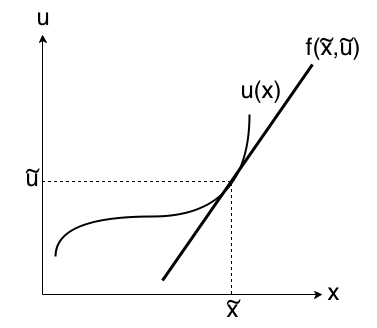
\includegraphics[scale=0.5]{pictures/011-04.png}
\end{center}
$(x, u, f(x,u)) $ heißt \emph{Richtungsfeld}. 
Ohne(!) Kenntnis der Umgebung gibt es einen Anstieg 
von $u(.)$ in $x$ für den Fall, dass $(x,u) $ zum 
Graphen von $u(.) $ gehört.
\begin{center}
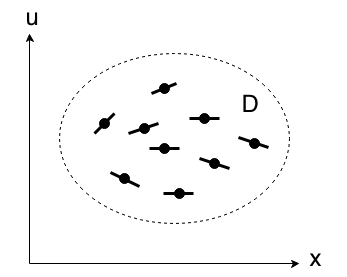
\includegraphics[scale=0.5]{pictures/011-05.png}
\end{center}
\emph{Problem:} Wir suchen die Kurve $u(.) $ die zum Richtungsfeld passt.\\
\emph{Anfangsgswert:} In 'vielen Fällen' geht durch jeden Punkt $(x,u) \in D $
        genau eine Kurve. Die Vorgabe 
        von $(x_0, u_0) = (x_0, u(x_0)) $ 
        liefert dann eine eindeutige Lösung.\\
        
        \emph{Näherungslösung:} Polygonzug\\
        Wir wählen $x_k = x_0 + k h$ mit ($\ k= 1 \ldots n, \ h$ - Schrittweite) und geben $u_0 = u(x_0) $ 
        wird Anfangswert vor.\\
\begin{center}
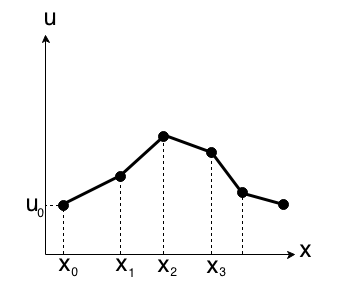
\includegraphics[scale=0.5]{pictures/011-06.png}
\end{center}
      
        
Die Schrittweise setzt man $u_k = u_{k+1} + h f(x_{k-1}, u_{k-1}), \ k= 1 \ldots n $. In 'vielen Fällen' konvergiert 
der Polygonzug für $h \rightarrow 0 $ gegen eine Lösung.
\item[ii)]$\mathbf{u'(x) = f(x)}$
        $\Rightarrow  u $ ist Stammfunktion von $f$
        Sei $f$ im Intervall $I \subset \mathbb{R} $ definiert und stetig, $x_0 \in I $\\
        Allgemeine Lösung: (vgl. Grundkurs)
\begin{equation*}
u(x) = \int\limits_{x_0}^x f(\xi) \mathrm{d}\xi + u_0, \ u_0 \in \mathbb{R}
\end{equation*}
Die Vorgabe $u_0$ entspricht gerade dem Anfangswert 
$u(x_0) = u_0 $.
    \item[iii)]$\mathbf{u'(x) = f(x) g(u(x))} $ ist eine 
    Differenzialgleichung mit getrennten Variablen. Wir 
    verwenden die folgende sogenannte \emph{Heuristik:}
\begin{equation*}
\diff{u}{x} = f(x) g(u) 
        \Rightarrow  \frac{1}{g(u)} \mathrm{d}u = f(x) \mathrm{d}x
\end{equation*}
Integration liefert dann
\begin{equation*}
\int \frac{1}{g(u)} \mathrm{d}u = \int f(x) \mathrm{d}x
\end{equation*}
um das Anfangswertproblem $u(x_0) = u_0 $ zu lösen, nehmen wir
\begin{equation}
\int\limits_{u_0}^u \frac{1}{g(s)} \mathrm{d}s 
= \int\limits_{x_0}^x f(x) \mathrm{d}x
\end{equation}
Auflösung nach $u$ liefert die Lösung $u = u(x)$.
        
\begin{beispiel*}
$u' = e^u \sin x, \ u(x_0) = u_0$ \\
Wenden wir die Heuristik an, so erhalten wir
\begin{equation*}
\int\limits_{u_0}^u e^{-s} \mathrm{d}s
        = \int\limits_{x_0}^x \sin \mathrm{d}t
\end{equation*}
\begin{equation*}
\left[ -e^{-s} \right]_{u_0}^u = \left[ - \cos t \right]_{x_0}^x \\
\end{equation*}
Das können wir dann schließlich noch umstellen
\begin{equation*}
\Rightarrow e^{-u} = \cos x - \cos x_0 + e^{-u_0}
\end{equation*}
\begin{equation*}
u(x) = -\ln ( \cos x 
        + \underbrace{e^{-u_0} - \cos x_0}_{\coloneqq c})
\end{equation*}        
\begin{center}
 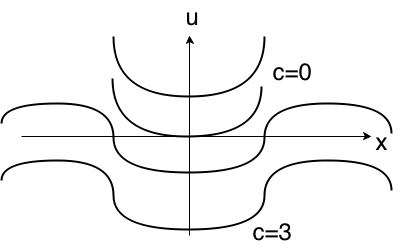
\includegraphics[scale=0.5]{pictures/011-07.png}
\end{center}        
       
        Es ist zu beachten, das sich abhängig von den 
        Anfangswerten der Definitionsbereich der
        Lösung ändert, wie zum Beispiel bei
        
        
\begin{equation*}
 u' = 
        \frac{
        \sin x}
        {\cos x + e^{-u_0} - \cos x_0}
        = e^u \sin x
\end{equation*}
        \end{beispiel*}        
